\section{PDEs in rectangular coordinates}

\subsection{Separation of variable for general equation}

In this section, we will consider separation of variable for more general equation, possibly with variable coefficients and more general boundary conditions. 

\subsubsection{Boundary conditions}

\textbf{TODO: as in ODE case, we need the boundary condition at any point on the boundary}

Given a PDE defined on a domain $R$, we must prescibe the boundary condition on $\partial R$.

\textbf{TODO: add $\partial R$ in the picture}
\begin{figure}[H]
    \scalebox{0.2}{      
        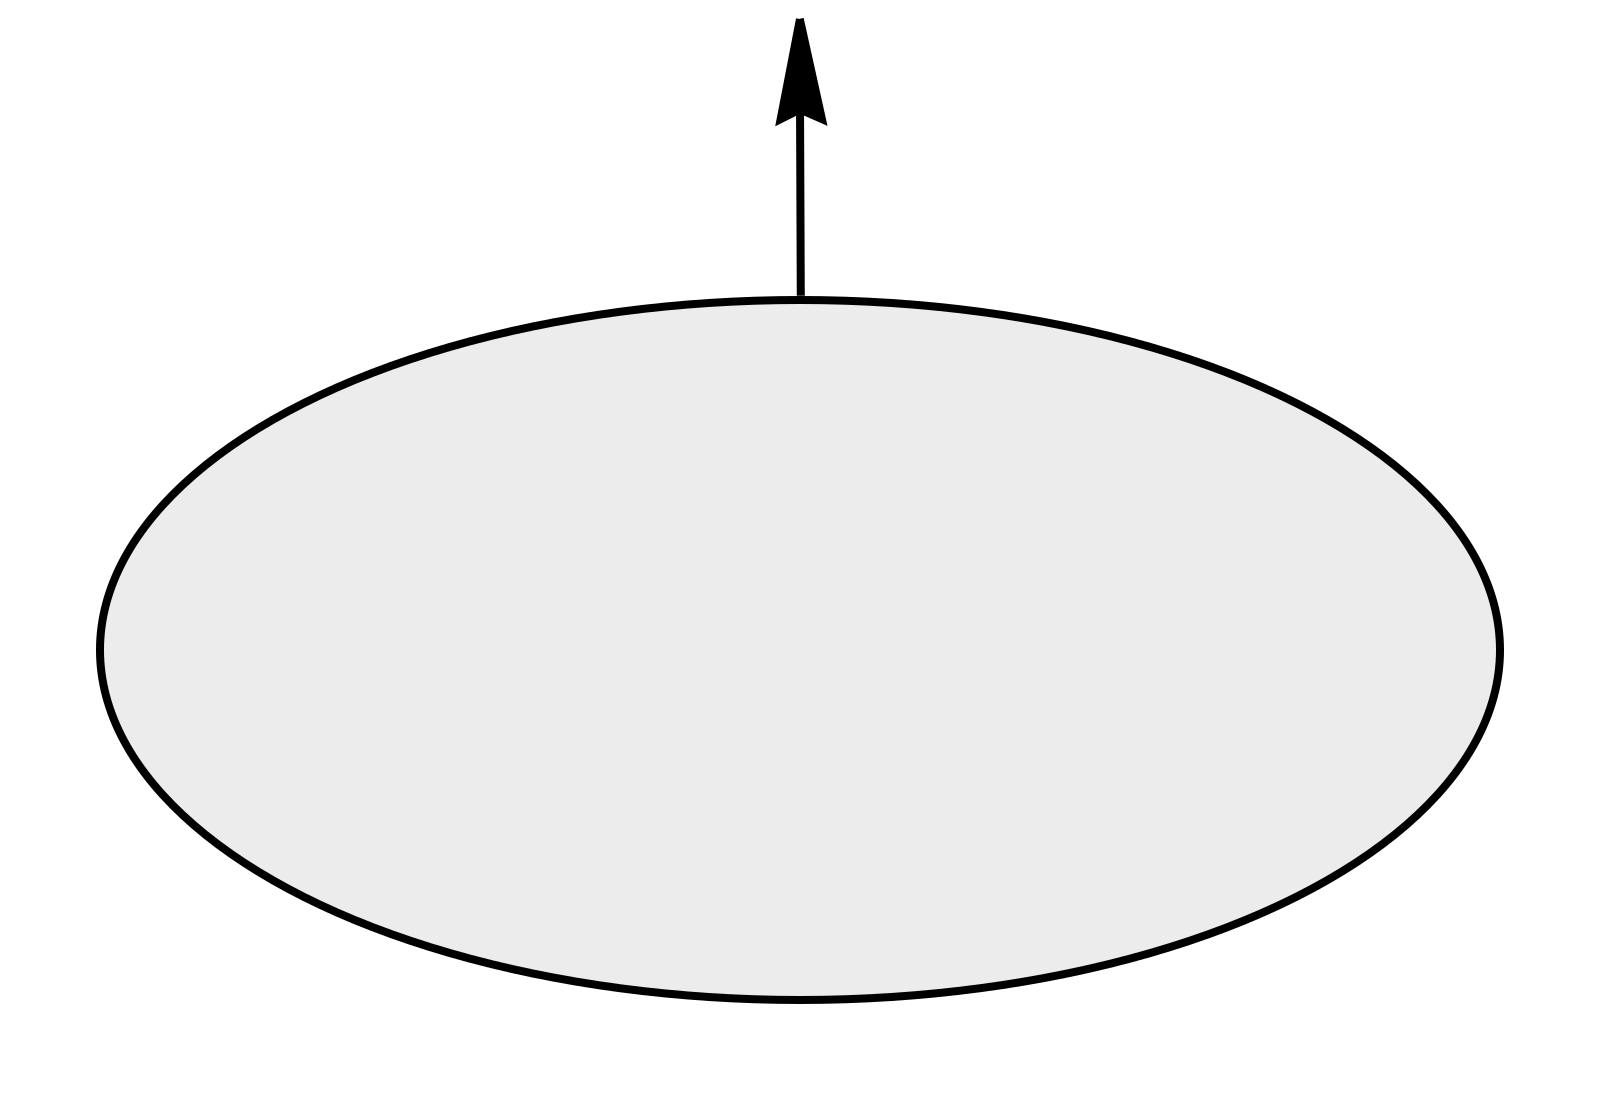
\includegraphics{pictures/normal_vector.png}
    }
    \centering 
    \caption{The region $R$ and its normal vector.} 
    \label{fig.normal_vector} 
\end{figure}

\textbf{TODO: explanation}

\begin{definition}[Normal vector] $\mathbf{n}$
    
\end{definition}

\begin{definition}[Boundary conditions] Consider a PDE $F[u] = 0$. Here are the boundary conditions that we consider in this class.
    \begin{enumerate}
        \item \textbf{Dirichlet boundary condition.} The value of $u$ on the boundary is given.
        \begin{equation}\label{eq.Dirichlet_boundary}
            u=g(x), \quad x \in \partial \Omega .
        \end{equation}
        
        \item \textbf{Neumann boundary condition.} The normal derivative on the boundary is given.
        \begin{equation}\label{eq.Neumann_boundary}
            \mathbf{n} \cdot \nabla u=g(x), \quad x \in \partial \Omega .
        \end{equation}
        
        \item \textbf{Robin boundary condition.} A linear combination of the above two boundary conditions. 
        \begin{equation}\label{eq.Robin_boundary}
            a(x) u+b(x) \mathbf{n} \cdot \nabla u=g(x), \quad x \in \partial \Omega .
        \end{equation}
    \end{enumerate}
\end{definition}

\subsubsection{Heat equations as an example}

\begin{figure}[H]
    \scalebox{0.15}{      
        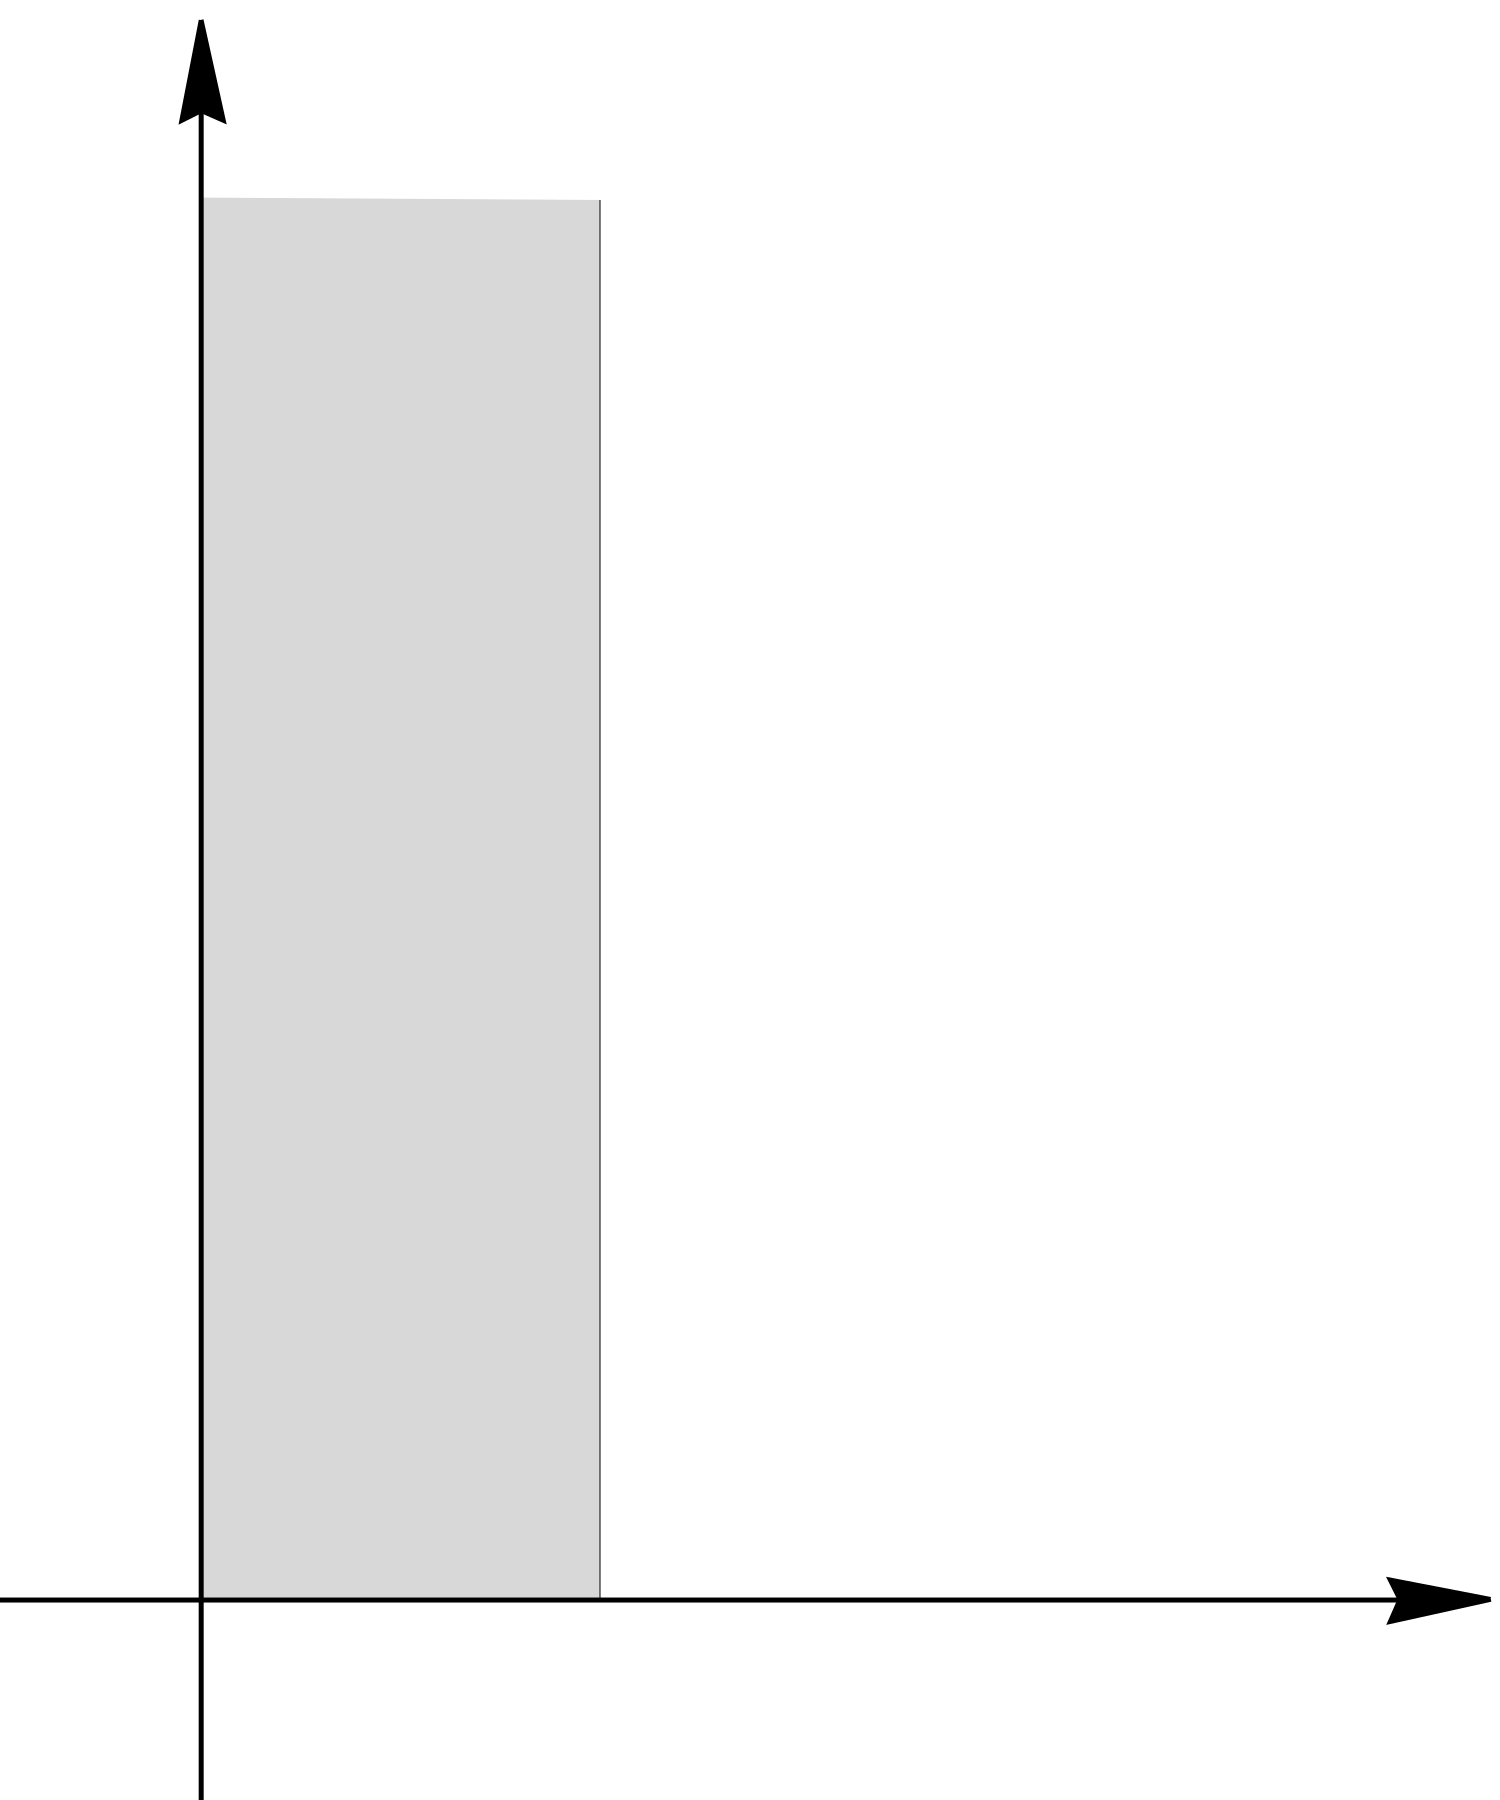
\includegraphics{pictures/heat_region.png}
    }
    \centering 
    \caption{The domain for the heat equation.} 
    \label{fig.heat_region} 
\end{figure}

\textbf{TODO: Robin, constant coefficients}

\textbf{TODO: compute the normal vector and simplify Robin}

\textbf{TODO: explain Dirichlet}

\textbf{TODO: second order need one condition but first order need one}

\begin{equation}
    \left\{\begin{aligned} 
        &u_t=K u_{z z}, && 0<z<L, \quad t>0, 
        \\ 
        &u \cos \alpha-L u_z \sin \alpha=0,\quad && z=0, \quad t>0, 
        \\ 
        &u \cos \beta+L u_z \sin \beta=0, && z=L, \quad t>0, 
        \\
        &u=f(z), && 0<z<L, \quad t=0,
    \end{aligned}\right.
\end{equation}

\textbf{TODO: add detail}



Let us solve the heat equation in a simple case of $\alpha=\beta=0$. The separated solution is written as $u(z, t)=\phi(z) T(t)$. Thus we obtain
$$
T^{\prime}(t)+\lambda K T(t)=0, \quad \phi^{\prime \prime}(z)+\lambda \phi(z)=0 .
$$

The boundary conditions are written as
$$
\phi(0)=\phi(L)=0 .
$$

We obtain
$$
T(t)=e^{-\lambda K t}, \quad \phi=A \sin (\sqrt{\lambda} z)+B \cos (\sqrt{\lambda} z), \quad \lambda>0 .
$$

By plugging $\phi=A \sin (\sqrt{\lambda} z)+B \cos (\sqrt{\lambda} z)$ into the boundary conditions, we find that $B=0$ and $\sqrt{\lambda} L$ is an integer multiple of $\pi$. Therefore we obtain
$$
\phi(z)=\phi_n(z)=\sin \left(\sqrt{\lambda_n} z\right), \quad \lambda_n=\left(\frac{n \pi}{L}\right)^2, \quad n=1,2, \ldots,
$$
where we set the arbitrary constant in $\phi_n(z)$ to be $1$ (recall we will take a superposition). Thus the separated solutions are obtained as
$$
u(z, t)=\phi_n(z) e^{-\lambda_n K t}, \quad n=1,2, \ldots
$$

If no initial condition is given, the above separated solutions are the solutions to the problem. Here, however, we have an initial condition.
Let us consider the initial condition. We express the solution as
$$
u(z, t)=\sum_{n=1}^{\infty} C_n \phi_n(z) e^{-\lambda_n K t},
$$
where $C_n$ are constants. Since $f$ is piecewise smooth, we can write $f(z)=\sum_{n=1}^{\infty} B_n \phi_n(z)$, $0<z<L$, with some coefficients $B_n$ (Fourier sine series). This implies that $C_n=B_n$. We obtain
$$
u(z, t)=\sum_{n=1}^{\infty} B_n \phi_n(z) e^{-\lambda_n K t}, \quad 0<z<L, \quad t>0 .
$$

\begin{example}[]
The heat equation $u_t=K u_{z z}$ for $0<z<L, t>0$ with $u(0, t)=u(L, t)=0$ and $u(z, 0)=1$ is solved as
$$
u(z, t)=\sum_{n=1}^{\infty} B_n \sin \frac{n \pi z}{L} e^{-(n \pi / L)^2 K t},
$$
where
$$
B_n=\frac{2}{\pi} \frac{1-(-1)^n}{n} .
$$

As mentioned above, $B_n$ are coefficients of the Fourier sine series of $f(z)$. We can also compute $B_n$ as follows. First, we note the following orthogonality relations. For $n, m=1,2, \ldots$, we have

\textbf{TODO: match boundary condition and using orthogonality}

\begin{equation*}
    \int_0^L \sin \frac{n \pi z}{L} \sin \frac{m \pi z}{L} d z = \frac{L}{2} \delta_{n m}
\end{equation*}
\end{example}

\subsubsection{Orthogonal functions}

\begin{definition}[Inner product] We extend dot product $\varphi \cdot \psi$ and define \underline{inner product} as
\begin{equation}\label{eq.inner_product}
    \langle\varphi, \psi\rangle=\int_a^b \varphi(x) \psi(x) d x .
\end{equation}
    
Sometimes the inner product is defined as follows. We can have a \underline{weight function} $\rho(x)$, and the weighted inner product is given by
\begin{equation}\label{eq.inner_product_weight}
    \langle\varphi, \psi\rangle_\rho=\int_a^b \varphi(x) \psi(x) \rho(x) d x
\end{equation}
where $\rho(x)>0$ is a weight function. 

For complex functions, we can write the \underline{complex inner product} as
\begin{equation}\label{eq.inner_product_complex}
    \langle\varphi, \psi\rangle=\int_a^b \varphi(x) \bar{\psi}(x) \rho(x) d x .
\end{equation}
Here $\bar{\psi}$ is the complex conjugate of $\psi$ $(\bar{\psi}(x)=f(x)-i g(x)$ when $\psi=f+i g)$.
    
\end{definition}

\begin{definition}[Orthogonality]
Two functions $\varphi, \psi$ are said to be \underline{orthogonal} on $[a, b]$ if $\langle\varphi, \psi\rangle=0$.    
\end{definition}

\begin{example}[]
    The functions $\varphi(x)=\sin x$ and $\psi(x)=\cos x$ are orthogonal on $[0, \pi]$.
\end{example}
\begin{example}[]
    The set of functions $\sin x, \sin 2 x, \ldots, \sin N x$ is orthogonal on $[0, \pi]$.
\end{example}
\begin{example}[]
    Which of the following pairs of functions are orthogonal on the interval $0 \leq x \leq 1$ ?
$$
\varphi_1=\sin 2 \pi x, \quad \varphi_2=x, \quad \varphi_3=\cos 2 \pi x, \quad \varphi_4=1 .
$$
$\left\langle\varphi_1, \varphi_3\right\rangle=0,\left\langle\varphi_1, \varphi_4\right\rangle=0,\left\langle\varphi_2, \varphi_3\right\rangle=0,\left\langle\varphi_3, \varphi_4\right\rangle=0$. All others are nonzero. Therefore the pairs $\left(\varphi_1, \varphi_3\right),\left(\varphi_1, \varphi_4\right),\left(\varphi_2, \varphi_3\right)$, and $\left(\varphi_3, \varphi_4\right)$ are orthogonal.
\end{example}

\begin{definition}[Norm]
As follows we define \underline{norm}, which is the ``length'' of a function.
$$
\|\varphi\|=\|\varphi\|_{L^2(a, b)}=\sqrt{\langle\varphi, \varphi\rangle} .
$$
We note that the norm is always nonnegative. The norm $\|\varphi-\psi\|$ is the distance between two functions $\varphi$ and $\psi$.
\end{definition}

\begin{definition}[Projection]
    Let $\left(\varphi_1, \ldots, \varphi_N\right)$ be a set of orthogonal functions with $\left\|\varphi_i\right\| \neq 0$. Let $f(x)$ be a function. Then $\hat{c}_1 \varphi_1+\cdots+\hat{c}_N \varphi_N$ with $\hat{c}_i=$ $\left\langle f, \varphi_i\right\rangle /\left\|\varphi_i\right\|^2$ is the projection of $f$ onto $\left(\varphi_1, \ldots, \varphi_N\right) . \hat{c}_i$ is called the $i$ th Fourier coefficient of $f$. 

    \textbf{TODO: revise this}
\end{definition}


Note that the minimum of $\left\|f-\left(c_1 \varphi_1+\cdots+c_N \varphi_N\right)\right\|$ is achieved when $c_i=\hat{c}_i$.
    
\begin{example}[]
    Find the projection of $f(x)=1$ onto $\left(\varphi_1, \varphi_2\right)=(\sin x, \sin 2 x)$ on the interval $0 \leq x \leq \pi$. By $\left\langle f, \varphi_1\right\rangle=2,\left\langle f, \varphi_2\right\rangle=0$, and $\left\|\varphi_1\right\|^2=\left\|\varphi_2\right\|^2=\frac{\pi}{2}$, we obtain $\frac{4}{\pi} \sin x$.   
\end{example}

\begin{definition}[Orthonormal]
    The functions $\left(\varphi_1, \ldots, \varphi_N\right)$ are orthonormal if $\left\langle\varphi_i, \varphi_j\right\rangle=$ $\delta_{i j}$. Here $\delta_{i j}$ is the Kronecker delta $(\delta_{i j}=0$ if $i \neq j$ and $=1$ if $i=j)$.
\end{definition}

\subsubsection{The Sturm-Liouville eigenvalue problem}

\subsubsection{Convergence of orthogonal series}

\subsection{The heat equation}

\subsubsection{Physics of heat conduction}

\subsubsection{The homogeneous case}

\subsubsection{The non-homogeneous case}

\subsection{The wave equation}

\subsubsection{Physics of string vibration}

\subsubsection{The homogeneous case}

\subsubsection{The non-homogeneous case}


\subsection{The Laplace's equation}

\subsubsection{Physics of static electricity}

\subsubsection{The homogeneous case}

\subsubsection{The non-homogeneous case}